\documentclass[aspectratio=169,11pt]{beamer}
\usetheme{default}
\usecolortheme{seagull}
\setbeamertemplate{navigation symbols}{}
\setbeamertemplate{footline}[frame number]
\setbeamerfont{frametitle}{size=\large,series=\bfseries}
\setbeamerfont{title}{size=\Large,series=\bfseries}
\usepackage{graphicx}
\graphicspath{{./}{../figures/}}
\newcommand{\src}[1]{\vfill{\tiny\textcolor{gray}{#1}}}

\title{T1K vs. Immuannot on the giraffe/whatshap 1000G pangenome-typing pipeline}
\author{Dawn Chen}
\institute{BioHackathon Japan 2026, HLA/pangenome group}
\date{16 September 2026}

\begin{document}

\begin{frame}
  \titlepage
\end{frame}

\begin{frame}{Four HLA typing runs on the same 1000G short-read cohort, compared pairwise}
  \begin{itemize}
    \item \textbf{t1k}: run-t1k directly on raw FASTQs extracted per sample from the 1000G high-coverage CRAMs (\texttt{mhc\_giraffe/t1k}); independent of the graph/phasing steps below
    \item \textbf{Immuannot, old DB}: vg giraffe alignment to leechuck's whole-MHC Minigraph-Cactus graph $\to$ \texttt{vg call} $\to$ WhatsHap read-backed phasing $\to$ \texttt{bcftools consensus} hap1/hap2 FASTAs $\to$ Immuannot against leechuck's frozen IPD-IMGT/HLA 3.55.0
    \item \textbf{Immuannot, new DB}: identical hap1/hap2 consensus FASTAs, re-annotated against a freshly built IPD-IMGT/HLA 3.65.0 (same release T1K uses) -- isolates database-version effects only
    \item \textbf{leechuck\_t1k}: leechuck's own run-t1k on raw 1000G reads, entirely outside this pipeline; 412 samples $\times$ 5 genes (A/B/C/DQB1/DRB1), merged against published truth genotypes
    \item Comparison: unordered allele pairs, truncated to 1-field (allele group) and 2-field (protein) resolution; Immuannot's \texttt{:new} suffix (no exact database match) stripped before truncation, not treated as a literal field
  \end{itemize}
\end{frame}

\begin{frame}{t1k and Immuannot each cover more than half of the 2,504-sample cohort so far}
  \centering
  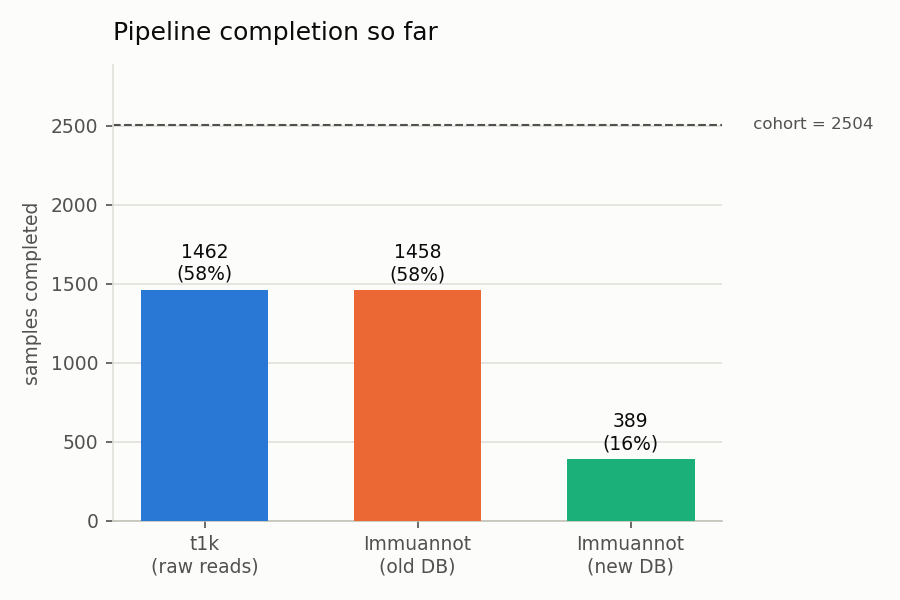
\includegraphics[width=0.54\textwidth]{gc_pipeline_completion.png}
  \begin{itemize}
    \item t1k and Immuannot-old-DB run independently per sample and finish at the same pace (both $\approx$ 58\%); Immuannot-new-DB is a smaller re-run launched later, still catching up (16\%)
    \item All figures on later slides use whatever fraction of the cohort had finished at the time of analysis
  \end{itemize}
\end{frame}

\begin{frame}{Immuannot's old and new databases agree almost perfectly; t1k agrees with Immuannot only 1 call in 3}
  \centering
  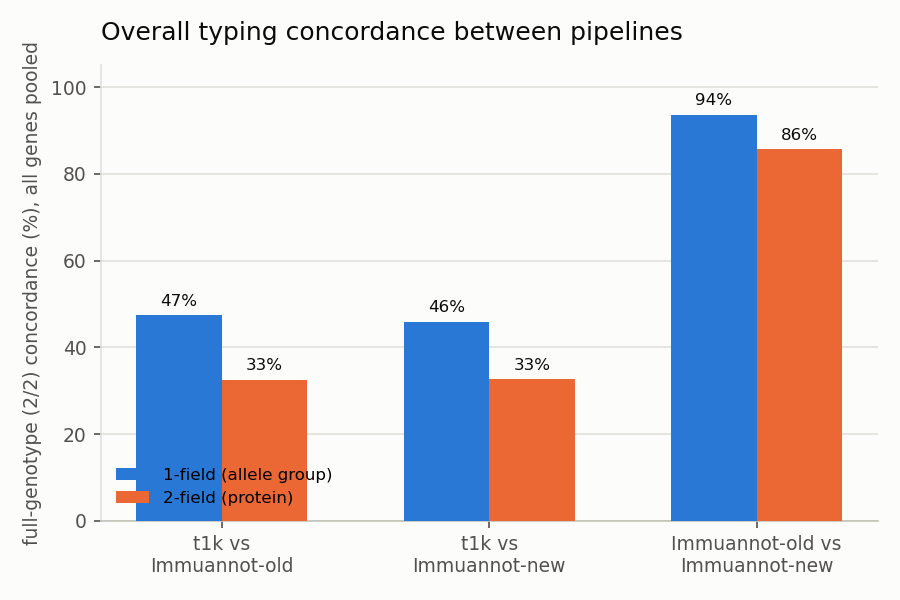
\includegraphics[width=0.56\textwidth]{gc_overall_concordance.png}
  \begin{itemize}\footnotesize
    \item Immuannot-old vs Immuannot-new: 86\% full-genotype (2-field), 94\% at 1-field -- expected, since it is the same consensus sequence, only the reference database changed
    \item t1k vs Immuannot (either DB): only $\approx$ 32\% full-genotype concordance -- Immuannot types off a phased short-read consensus (subject to phasing/assembly error), t1k types straight from reads
  \end{itemize}
\end{frame}

\begin{frame}{HLA-DRB1 concordance collapses in every pairwise comparison}
  \centering
  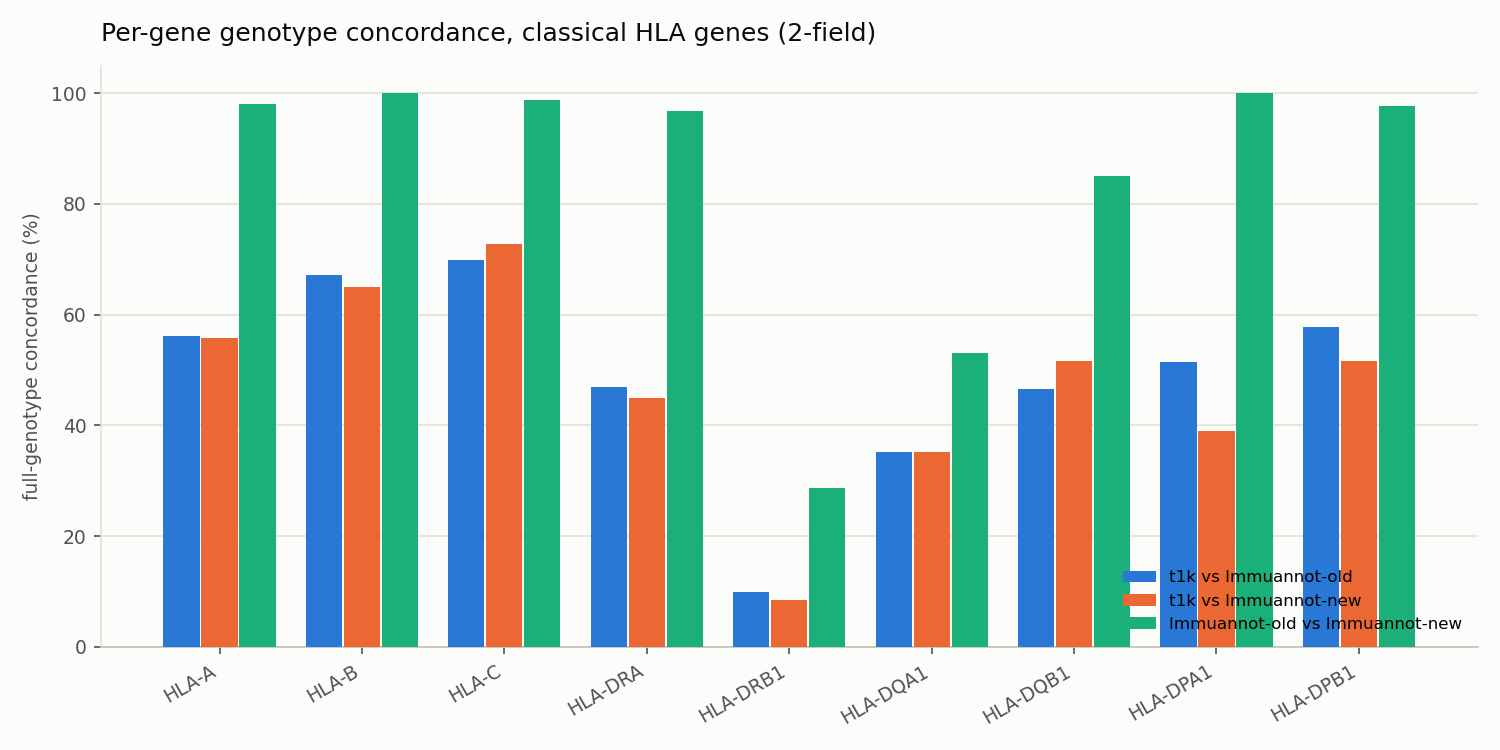
\includegraphics[width=0.82\textwidth]{gc_per_gene_concordance.png}
  \begin{itemize}\small
    \item A/B/C/DPA1/DPB1: Immuannot-old vs Immuannot-new $\ge$ 97\%; t1k vs either Immuannot 50--74\%
    \item HLA-DRB1: only 9--29\% concordance for every pair, including Immuannot-old vs Immuannot-new (same consensus sequence!) -- a paralog-confusable, hard-to-phase locus, not a database-version or typer artifact
  \end{itemize}
\end{frame}

\begin{frame}{How: genotype comparison at 1- and 2-field resolution}
  \begin{itemize}
    \item Truncate each allele string to its first ($k{=}1$) or first two ($k{=}2$) colon-separated fields after the gene, e.g. \texttt{HLA-A*29:02:01:01} $\to$ \texttt{HLA-A*29:02}
    \item Immuannot's \texttt{:new} suffix marks the point past which no exact database allele matched -- \texttt{HLA-A*01:new} is only \emph{1-field}-resolved, not a literal second field of ``new''; stripped before truncation, and a 2-field comparison is skipped (not counted as a mismatch) when fewer than 2 real fields remain
    \item Genotype match: best of the two possible allele-pairings (hap1/hap2 vs allele1/allele2 order is arbitrary between pipelines); full match requires 2/2 alleles to agree
    \item Script: \texttt{analysis/gc\_typing\_concordance.py}; tables in \texttt{results/tables/gc\_*.tsv}
  \end{itemize}
\end{frame}

\begin{frame}{65--88\% of Immuannot's classical-gene calls are novel (\texttt{:new}), consistent with imperfect short-read phasing}
  \centering
  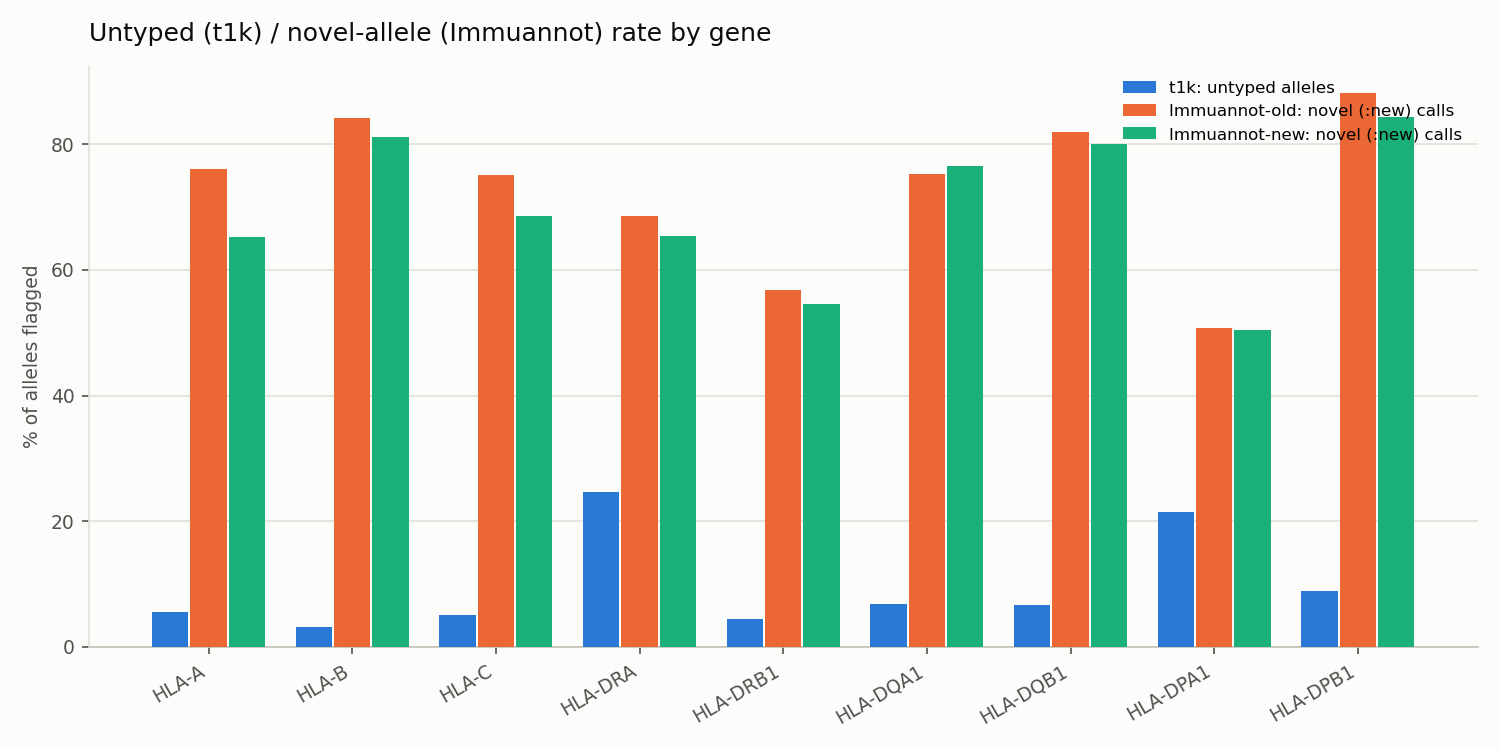
\includegraphics[width=0.7\textwidth]{gc_novel_uncalled_rate.png}
  \begin{itemize}\footnotesize
    \item t1k rarely leaves a classical gene untyped (3--9\%, DPA1/DRA higher at 21--25\% -- both have many database alleles close in sequence)
    \item Immuannot flags a novel allele on 65--88\% of A/B/C/DQB1/DPB1 calls, old and new DB alike -- the consensus sequence itself, not the database, is the limiting factor (matches the pipeline's own documented caveat: WhatsHap phasing can leave chimeric/ambiguous consensus for highly polymorphic genes)
  \end{itemize}
\end{frame}

\begin{frame}{leechuck's raw-read t1k agrees with Immuannot far better than this pipeline's own t1k does}
  \centering
  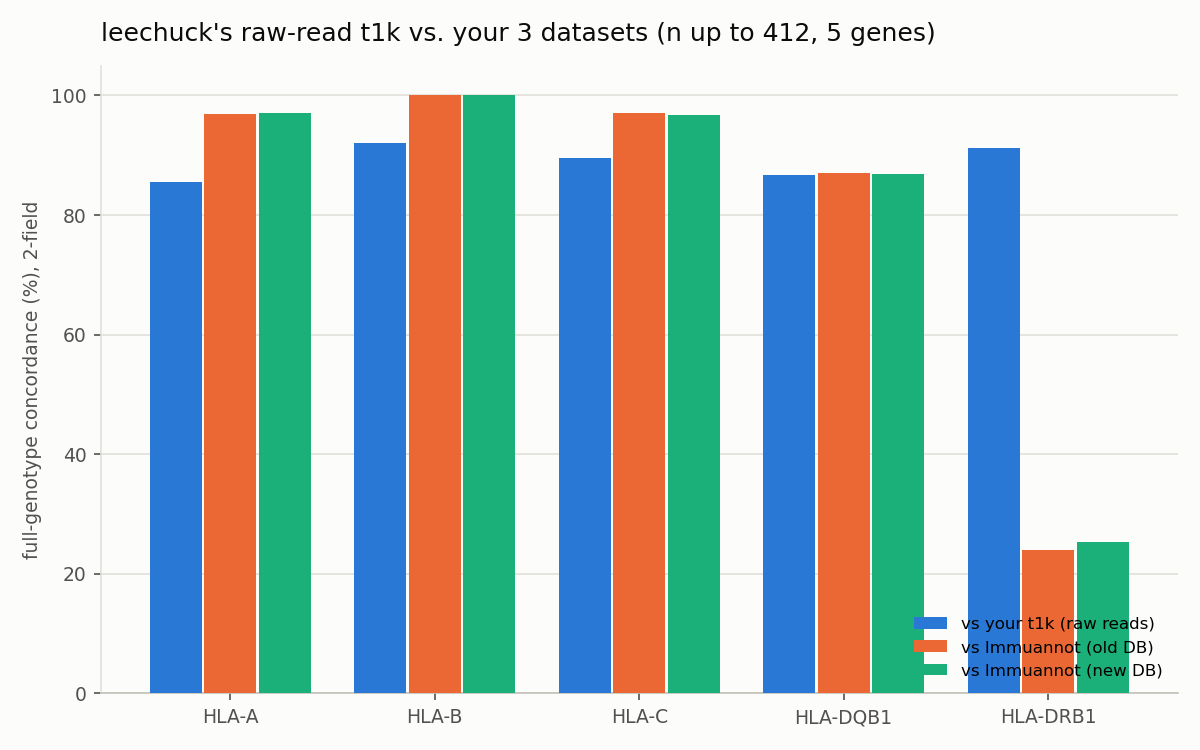
\includegraphics[width=0.5\textwidth]{gc_leechuck_t1k_comparison.png}
  \begin{itemize}\footnotesize
    \item Same 5 genes, up to 412 samples (different, smaller subset than the whole-cohort figures above)
    \item vs. this pipeline's t1k: 85--92\% -- the two t1k runs mostly agree with each other
    \item vs. Immuannot (either DB): 87--100\% for A/B/C/DQB1 -- markedly higher than this pipeline's own t1k-vs-Immuannot ($\approx$ 54--70\% on these genes, previous whole-cohort figures); DRB1 still collapses (24--25\%)
    \item Read: when the two t1k runs disagree, it is usually this pipeline's t1k that is the outlier relative to Immuannot -- investigated on the next slide
  \end{itemize}
\end{frame}

\begin{frame}{Digging in: same t1k binary, same database, different read extraction}
  \begin{itemize}
    \item Both t1k runs use the identical database: \texttt{diff} of the two \texttt{hlaidx\_dna\_seq.fa} files (29,429 alleles each, IPD-IMGT/HLA 3.65.0) is non-empty only because records are in a different order -- sorted, byte-identical. Rules out a database-version explanation
    \item mhc\_pipeline.sbatch's t1k step even reuses leechuck's own conda env (\texttt{mm/envs/typing/bin}) -- same t1k version too
    \item Where they differ: \textbf{read extraction}. leechuck's \texttt{kg\_mhc\_reads.sbatch} pulls reads aligned to the MHC region \emph{and} the 16 GRCh38 \texttt{chr6\_*\_alt} contigs \emph{and} the 525 \texttt{HLA-*} allele contigs (542 regions total) straight from the 1000G high-coverage CRAMs
    \item This pipeline's extraction (\texttt{03\_subsample\_1000g\_cram.sh}) pulls the MHC region and the 525 \texttt{HLA-*} contigs, but \emph{not} the 16 \texttt{chr6\_*\_alt} contigs (it adds unmapped reads instead, which leechuck's does not)
  \end{itemize}
\end{frame}

\begin{frame}{Root cause: this pipeline's read extraction misses the chr6 MHC ALT haplotype contigs}
  \begin{itemize}\small
    \item Checked directly on HG00097 (one of the discordant samples, homozygous in leechuck's t1k, one allele untyped in ours): \textbf{224,460 reads} in its 1000G CRAM align to the 16 \texttt{chr6\_*\_alt} contigs alone
    \item Those reads never reach this pipeline's t1k input at all -- for a sample whose true haplotype is closer to an ALT scaffold than to the GRCh38 primary path, this can substantially reduce effective read support for the divergent allele
    \item Consistent with the observed failure mode: t1k calls one allele confidently and either repeats it (leechuck, full read set) or leaves the second slot untyped (ours, reduced read set) -- an abundance/coverage effect, not a wrong call
    \item Fix: add the 16 \texttt{chr6\_*\_alt} contigs to \texttt{hla\_decoy\_contigs.txt} / the extraction region list and re-run t1k; cheap, since it only touches the read-extraction step
  \end{itemize}
\end{frame}

\begin{frame}{Take-home}
  \begin{itemize}\small
    \item Immuannot's database version (3.55 vs 3.65) barely matters here (86--94\% agreement); the consensus sequence quality from graph alignment + WhatsHap phasing is the real bottleneck, especially for A/B/C/DQB1/DPB1 (65--88\% flagged novel) and DRB1 (concordance collapses even DB-vs-DB)
    \item t1k-vs-Immuannot discordance ($\approx$ 32\% whole-cohort) is expected and matches the pipeline's own documented caveat about imperfect phasing -- t1k is the more trustworthy call for benchmarking, per that same caveat
    \item A second, independent t1k run (leechuck's) agrees with Immuannot noticeably better than this pipeline's t1k does; traced to a read-extraction gap (missing chr6 MHC ALT contigs), not a tool, database, or pangenome-pipeline difference -- fixable
    \item Open: re-run this pipeline's read extraction with the ALT contigs included and re-check t1k-vs-leechuck\_t1k concordance; revisit DRB1 specifically once Immuannot-new-DB finishes the full cohort
    \item Script, figures, tables: \texttt{pangenome-bh26/hla/analysis/gc\_typing\_concordance.py}, \texttt{results/figures/gc\_*.png}, \texttt{results/tables/gc\_*.tsv}
  \end{itemize}
\end{frame}

\end{document}
